\documentclass[12pt]{article}
%Gumm{\color{blue}i}|065|=)
\usepackage{amsmath, amsfonts, amssymb}
\usepackage[margin=0.5in]{geometry}
\usepackage{xcolor}
\usepackage{graphicx}
\usepackage{amsmath}

\newcommand{\off}[1]{}
\DeclareMathSizes{20}{30}{20}{18}
\usepackage{tikz}


\title{Scratchwork: Schemes}
\date{}
\begin{document}

\sffamily

\maketitle

\noindent 
Let's list some of the examples in Chapter 2 of \textbf{Geometry fo Schemes}
\begin{itemize}
\item $\text{Spec}\;R$ with $R = \mathbb{K}[x,y]/(x^2, xy, y^2, ax+by) \simeq K[t]/(t^2)$ This is a double-point.
\item $\text{Spec}K[x]/(x^3) \not\simeq \text{Spec}K[x,y]/(x^2,xy,y^2)$.  These are examles of triple-points.
\item $X_t = \{ (0,0), (t,0), (0,t) \} \subset \mathbb{A}_K^2$ be three points in the affine plane $\mathbb{A}_K$.  The limit scheme as $t \to 0$ is:
$$ \lim_{t \to 0} X_t = X_0 = \text{Spec}K[x,y]/(x^2, xy, y^2) $$
which is a triple-point. There were three points to begin with and now they are infinitesimally close together. 
\end{itemize}
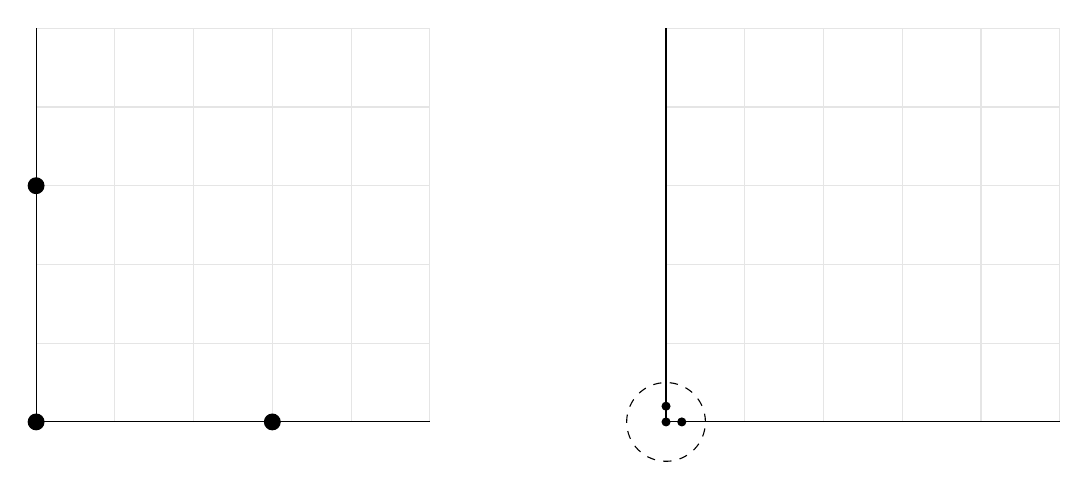
\begin{tikzpicture}
\begin{scope}[xshift=0]

\foreach \a in {0,...,5}{

\draw[black!10!white] (0,\a)--(5,\a);
\draw[black!10!white] (\a,0)--(\a,5);
}

\draw (0,0)--(5,0);
\draw (0,0)--(0,5);
\draw[fill=black] (0,0) circle (0.1);
\draw[fill=black] (0,3) circle (0.1);
\draw[fill=black] (3,0) circle (0.1);



\end{scope}

\begin{scope}[xshift=8cm]

\foreach \a in {0,...,5}{

\draw[black!10!white] (0,\a)--(5,\a);
\draw[black!10!white] (\a,0)--(\a,5);
}

\draw (0,0)--(5,0);
\draw (0,0)--(0,5);
\draw[fill=black] (0,0) circle (0.05);
\draw[fill=black] (0,0.2) circle (0.05);
\draw[fill=black] (0.2,0) circle (0.05);
\draw[dashed] (0,0) circle (0.5);
\end{scope}
\end{tikzpicture} \\
Even more examples:
\begin{itemize}
\item $X = \text{Spec} K[x,y] = (x^2y, xy^2)$ the union of the $x$-axis and the $y$-axis. $\{ x = 0 \} \cup \{ y = 0 \}$.
\end{itemize}
Due to our lack of imagination, these are the minimum we can do.  These arise as limiting situations in classical geometry and we are advised to look at a high-school textbook from here. 
\vfill
\begin{thebibliography}{} 

\item Henri Cohen \textbf{Computational Number Theory in Relation with L-Functions} \texttt{arXiv:1809.10904}

\item Hugh Montgomery, Robert Vaughan \textbf{Multiplicative Number Theory I: Classical Theory} \\ (Cambridge Studies in Advanced Mathematics, \#97) Cambridge University Press, 2010.

\item Yitzhak Katznelson \textbf{An Introduction to Harmonic Analysis} (Cambridge Mathematical Library) \\ Cambridge University Press, 2004.

\end{thebibliography}

\begin{thebibliography}{} 

\item David Eisenbud, Joe Harris.  \textbf{The Geometry of Schemes}. (GTM \#197) Springer, 2000.
\item Ravi Vakil \textbf{Foundations of Algebraic Geometry} (online) \texttt{http://math.stanford.edu/~vakil/216blog/}

\end{thebibliography}

\newpage

\noindent \textbf{12/03/18} Schemes are meant to capture reasonable things that fail to be varieties.  Let's try two examples.  \\ \\
\textbf{1} The rational points on a circle.  $X(\mathbb{Q}) = \{ x^2 + y^2 - 1 = 0 \} \subseteq \mathbb{Q}^2$.  The definitions identify for us some choices we have made, in between the lines.  Our choice of ambient space, $\mathbb{A}_\mathbb{Q}^2 \simeq \mathbb{Q}^2$ is as good as any.  We could have chosen to place our circle as the a great circle in a sphere $X_1 = \{ x^2 + y^2 + z^2 - 1 = 0\}$ or in a cone $X_2 = \{ x^2 + y^2 = z^2 \}$.  Since we have restricted ourselves to the field of rational numbers $\mathbb{Q}$.  \\ \\
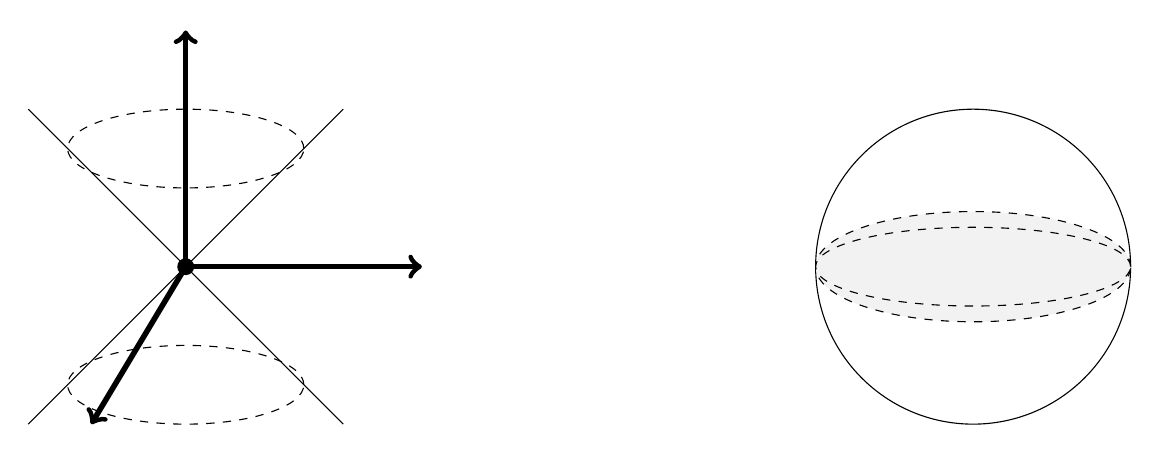
\begin{tikzpicture}[scale=2]

\begin{scope}
\draw (-1,-1)--(1,1);
\draw (-1,1)--(1,-1);

\draw[dashed] (0, 0.75) ellipse (0.75 and 0.25);
\draw[dashed] (0,-0.75) ellipse (0.75 and 0.25);

\draw[fill=black] (0,0) circle (0.05);

\draw[->, line width=2] (0,0)--(1.5,0);
\draw[->, line width=2] (0,0)--(0,1.5);
\draw[->, line width=2] (0,0)--(-0.6,-1);
\end{scope}

\begin{scope}[xshift=5cm]
\draw (0,0) circle (1);
\draw[dashed, fill=black!5!white] (0,0) ellipse (1 and 0.35);
\draw[dashed, fill=black!5!white] (0,0) ellipse (1 and 0.25);
\end{scope}

\end{tikzpicture}\\ \\
\textbf{Exercise:} Correct the two drawings above. Left: draw axes with proper perspective. Right: two nearby circles. Both: corrctly draw rational points on the sphere and cone.\\ \\
\textbf{2} While circles are an idealization, these shape remain the standard for measuring distance of any kind, as reference points or templates.  Thefore, it behooves us to understand how two circles intersect, or how these intersection points change when moved. \\
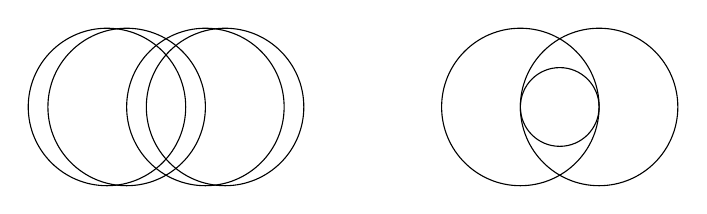
\begin{tikzpicture}
\begin{scope}
\draw ( 0.5,0) circle (1);
\draw (-0.5,0) circle (1);

\draw ( 0.5+0.25,0) circle (1);
\draw (-0.5-0.25,0) circle (1);
\end{scope}

\begin{scope}[xshift=5cm]
\draw ( 0.5,0) circle (1);
\draw (-0.5,0) circle (1);
\draw (0,0) circle (0.5);
\end{scope}
\end{tikzpicture} \\
\textbf{Exercise:} Compute the intersection points.  Do these points live in $\mathbb{Q}^2$? How do the intersecion points move as we move the circles left and right?

\vfill

\begin{thebibliography}{} 

\item David Eisenbud \textbf{3264 and All That} Cambridge University Press, 2016.
\item J. Rafael Sendra, Franz Winkler, Sonia Pérez-Díaz \textbf{Rational Algebraic Curves
A Computer Algebra Approach} (Algorithms and Computation in Mathematics \#22) Springer, 2008.
\item Donu Arapura \textbf{Algebraic Geometry over the Complex Numbers} (Universitext) Springer, 2012.

\item Yuri Manin \textbf{Introduction to the Theory of Schemes} (Moscow Lecture \#1) Springer, 2018.

\end{thebibliography}

\newpage

\noindent \textbf{3} If we make a mistake in our circle equation\footnote{By ``variety" I mean ``scheme" or ``sheaf" or some other equation-like thing.}, and only have $\{x^2 + y^2 -1 \approx 0\}$ can we still have an algebraic variety over $\mathbb{Q}$. \\
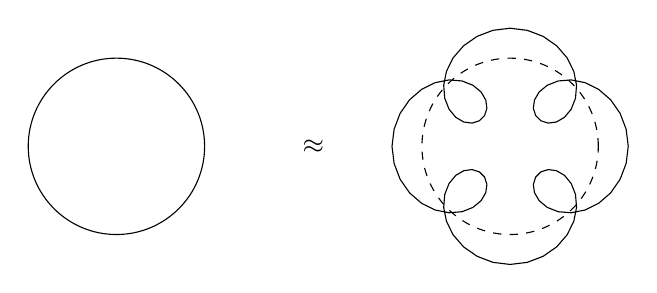
\begin{tikzpicture}
\begin{scope}
\draw ( 0,0) circle (1.12);
\end{scope}

\begin{scope}[xshift=2.5cm]
\node at (0,0) {$\approx$};
\end{scope}

\begin{scope}[xshift=5cm]

\draw[dashed] ( 0,0) circle (1.12);

\draw (1.5,0.0)--(1.47355498658,0.217299016717)--(1.3966231985,0.419225859711)--(1.27617987687,0.591889811773)--(1.12309165832,0.724218145312)--(0.951056516295,0.809016994375)--(0.775267988701,0.843652810832)--(0.61093442632,0.830287788753)--(0.471798182856,0.775646300248)--(0.368799667354,0.690335292166)--(0.309016994375,0.587785252292)--(0.294984984628,0.482915492561)--(0.324460130234,0.390654479782)--(0.390654479782,0.324460130234)--(0.482915492561,0.294984984628)--(0.587785252292,0.309016994375)--(0.690335292166,0.368799667354)--(0.775646300248,0.471798182856)--(0.830287788753,0.61093442632)--(0.843652810832,0.775267988701)--(0.809016994375,0.951056516295)--(0.724218145312,1.12309165832)--(0.591889811773,1.27617987687)--(0.419225859711,1.3966231985)--(0.217299016717,1.47355498658)--(2.14313189851e-16,1.5)--(-0.217299016717,1.47355498658)--(-0.419225859711,1.3966231985)--(-0.591889811773,1.27617987687)--(-0.724218145312,1.12309165832)--(-0.809016994375,0.951056516295)--(-0.843652810832,0.775267988701)--(-0.830287788753,0.61093442632)--(-0.775646300248,0.471798182856)--(-0.690335292166,0.368799667354)--(-0.587785252292,0.309016994375)--(-0.482915492561,0.294984984628)--(-0.390654479782,0.324460130234)--(-0.324460130234,0.390654479782)--(-0.294984984628,0.482915492561)--(-0.309016994375,0.587785252292)--(-0.368799667354,0.690335292166)--(-0.471798182856,0.775646300248)--(-0.61093442632,0.830287788753)--(-0.775267988701,0.843652810832)--(-0.951056516295,0.809016994375)--(-1.12309165832,0.724218145312)--(-1.27617987687,0.591889811773)--(-1.3966231985,0.419225859711)--(-1.47355498658,0.217299016717)--(-1.5,4.28626379702e-16)--(-1.47355498658,-0.217299016717)--(-1.3966231985,-0.419225859711)--(-1.27617987687,-0.591889811773)--(-1.12309165832,-0.724218145312)--(-0.951056516295,-0.809016994375)--(-0.775267988701,-0.843652810832)--(-0.61093442632,-0.830287788753)--(-0.471798182856,-0.775646300248)--(-0.368799667354,-0.690335292166)--(-0.309016994375,-0.587785252292)--(-0.294984984628,-0.482915492561)--(-0.324460130234,-0.390654479782)--(-0.390654479782,-0.324460130234)--(-0.482915492561,-0.294984984628)--(-0.587785252292,-0.309016994375)--(-0.690335292166,-0.368799667354)--(-0.775646300248,-0.471798182856)--(-0.830287788753,-0.61093442632)--(-0.843652810832,-0.775267988701)--(-0.809016994375,-0.951056516295)--(-0.724218145312,-1.12309165832)--(-0.591889811773,-1.27617987687)--(-0.419225859711,-1.3966231985)--(-0.217299016717,-1.47355498658)--(-1.53111798925e-15,-1.5)--(0.217299016717,-1.47355498658)--(0.419225859711,-1.3966231985)--(0.591889811773,-1.27617987687)--(0.724218145312,-1.12309165832)--(0.809016994375,-0.951056516295)--(0.843652810832,-0.775267988701)--(0.830287788753,-0.61093442632)--(0.775646300248,-0.471798182856)--(0.690335292166,-0.368799667354)--(0.587785252292,-0.309016994375)--(0.482915492561,-0.294984984628)--(0.390654479782,-0.324460130234)--(0.324460130234,-0.390654479782)--(0.294984984628,-0.482915492561)--(0.309016994375,-0.587785252292)--(0.368799667354,-0.690335292166)--(0.471798182856,-0.775646300248)--(0.61093442632,-0.830287788753)--(0.775267988701,-0.843652810832)--(0.951056516295,-0.809016994375)--(1.12309165832,-0.724218145312)--(1.27617987687,-0.591889811773)--(1.3966231985,-0.419225859711)--(1.47355498658,-0.217299016717)--(1.5,-8.57252759403e-16)--cycle; 

\end{scope} 
\end{tikzpicture} \\ 
Schemes are are necessary to describe the complicated intersections for the rose curves above.  This drawing arises in the plausiable-looking approximation:
$$ e^{i\theta} \approx e^{i\theta} \big( 1  + 0.25\, e^{4i\theta} \big) $$
Bounds for rational points on varieties and schemes has been done in many places, but it remains to find an elementary description of this points, avoiding the ineviable complicated mess.  The radius is $\sqrt{1 + 0.25^2} \approx 1.12$. \\ \\
\textbf{Exercise:} If you take their word for it, this is a genus $=0$ curve and has a ratioinal parameterization.  Find the rational points on this rose curve, and discuss the relevant action of $\mathbb{Q}^\times$.

\begin{thebibliography}{} 

\item Sophie Morel \textit{Introduction to Derived Algebraic Geometry} (course notes in French, unfinished)\\ \texttt{https://web.math.princeton.edu/\~{}smorel/notes.pdf}

\end{thebibliography}

\end{document}